% Options for packages loaded elsewhere
\PassOptionsToPackage{unicode}{hyperref}
\PassOptionsToPackage{hyphens}{url}
%
\documentclass[
  man]{apa6}
\usepackage{amsmath,amssymb}
\usepackage{iftex}
\ifPDFTeX
  \usepackage[T1]{fontenc}
  \usepackage[utf8]{inputenc}
  \usepackage{textcomp} % provide euro and other symbols
\else % if luatex or xetex
  \usepackage{unicode-math} % this also loads fontspec
  \defaultfontfeatures{Scale=MatchLowercase}
  \defaultfontfeatures[\rmfamily]{Ligatures=TeX,Scale=1}
\fi
\usepackage{lmodern}
\ifPDFTeX\else
  % xetex/luatex font selection
\fi
% Use upquote if available, for straight quotes in verbatim environments
\IfFileExists{upquote.sty}{\usepackage{upquote}}{}
\IfFileExists{microtype.sty}{% use microtype if available
  \usepackage[]{microtype}
  \UseMicrotypeSet[protrusion]{basicmath} % disable protrusion for tt fonts
}{}
\makeatletter
\@ifundefined{KOMAClassName}{% if non-KOMA class
  \IfFileExists{parskip.sty}{%
    \usepackage{parskip}
  }{% else
    \setlength{\parindent}{0pt}
    \setlength{\parskip}{6pt plus 2pt minus 1pt}}
}{% if KOMA class
  \KOMAoptions{parskip=half}}
\makeatother
\usepackage{xcolor}
\usepackage{graphicx}
\makeatletter
\def\maxwidth{\ifdim\Gin@nat@width>\linewidth\linewidth\else\Gin@nat@width\fi}
\def\maxheight{\ifdim\Gin@nat@height>\textheight\textheight\else\Gin@nat@height\fi}
\makeatother
% Scale images if necessary, so that they will not overflow the page
% margins by default, and it is still possible to overwrite the defaults
% using explicit options in \includegraphics[width, height, ...]{}
\setkeys{Gin}{width=\maxwidth,height=\maxheight,keepaspectratio}
% Set default figure placement to htbp
\makeatletter
\def\fps@figure{htbp}
\makeatother
\setlength{\emergencystretch}{3em} % prevent overfull lines
\providecommand{\tightlist}{%
  \setlength{\itemsep}{0pt}\setlength{\parskip}{0pt}}
\setcounter{secnumdepth}{-\maxdimen} % remove section numbering
% Make \paragraph and \subparagraph free-standing
\ifx\paragraph\undefined\else
  \let\oldparagraph\paragraph
  \renewcommand{\paragraph}[1]{\oldparagraph{#1}\mbox{}}
\fi
\ifx\subparagraph\undefined\else
  \let\oldsubparagraph\subparagraph
  \renewcommand{\subparagraph}[1]{\oldsubparagraph{#1}\mbox{}}
\fi
\newlength{\cslhangindent}
\setlength{\cslhangindent}{1.5em}
\newlength{\csllabelwidth}
\setlength{\csllabelwidth}{3em}
\newlength{\cslentryspacingunit} % times entry-spacing
\setlength{\cslentryspacingunit}{\parskip}
\newenvironment{CSLReferences}[2] % #1 hanging-ident, #2 entry spacing
 {% don't indent paragraphs
  \setlength{\parindent}{0pt}
  % turn on hanging indent if param 1 is 1
  \ifodd #1
  \let\oldpar\par
  \def\par{\hangindent=\cslhangindent\oldpar}
  \fi
  % set entry spacing
  \setlength{\parskip}{#2\cslentryspacingunit}
 }%
 {}
\usepackage{calc}
\newcommand{\CSLBlock}[1]{#1\hfill\break}
\newcommand{\CSLLeftMargin}[1]{\parbox[t]{\csllabelwidth}{#1}}
\newcommand{\CSLRightInline}[1]{\parbox[t]{\linewidth - \csllabelwidth}{#1}\break}
\newcommand{\CSLIndent}[1]{\hspace{\cslhangindent}#1}
\ifLuaTeX
\usepackage[bidi=basic]{babel}
\else
\usepackage[bidi=default]{babel}
\fi
\babelprovide[main,import]{english}
% get rid of language-specific shorthands (see #6817):
\let\LanguageShortHands\languageshorthands
\def\languageshorthands#1{}
% Manuscript styling
\usepackage{upgreek}
\captionsetup{font=singlespacing,justification=justified}

% Table formatting
\usepackage{longtable}
\usepackage{lscape}
% \usepackage[counterclockwise]{rotating}   % Landscape page setup for large tables
\usepackage{multirow}		% Table styling
\usepackage{tabularx}		% Control Column width
\usepackage[flushleft]{threeparttable}	% Allows for three part tables with a specified notes section
\usepackage{threeparttablex}            % Lets threeparttable work with longtable

% Create new environments so endfloat can handle them
% \newenvironment{ltable}
%   {\begin{landscape}\centering\begin{threeparttable}}
%   {\end{threeparttable}\end{landscape}}
\newenvironment{lltable}{\begin{landscape}\centering\begin{ThreePartTable}}{\end{ThreePartTable}\end{landscape}}

% Enables adjusting longtable caption width to table width
% Solution found at http://golatex.de/longtable-mit-caption-so-breit-wie-die-tabelle-t15767.html
\makeatletter
\newcommand\LastLTentrywidth{1em}
\newlength\longtablewidth
\setlength{\longtablewidth}{1in}
\newcommand{\getlongtablewidth}{\begingroup \ifcsname LT@\roman{LT@tables}\endcsname \global\longtablewidth=0pt \renewcommand{\LT@entry}[2]{\global\advance\longtablewidth by ##2\relax\gdef\LastLTentrywidth{##2}}\@nameuse{LT@\roman{LT@tables}} \fi \endgroup}

% \setlength{\parindent}{0.5in}
% \setlength{\parskip}{0pt plus 0pt minus 0pt}

% Overwrite redefinition of paragraph and subparagraph by the default LaTeX template
% See https://github.com/crsh/papaja/issues/292
\makeatletter
\renewcommand{\paragraph}{\@startsection{paragraph}{4}{\parindent}%
  {0\baselineskip \@plus 0.2ex \@minus 0.2ex}%
  {-1em}%
  {\normalfont\normalsize\bfseries\itshape\typesectitle}}

\renewcommand{\subparagraph}[1]{\@startsection{subparagraph}{5}{1em}%
  {0\baselineskip \@plus 0.2ex \@minus 0.2ex}%
  {-\z@\relax}%
  {\normalfont\normalsize\itshape\hspace{\parindent}{#1}\textit{\addperi}}{\relax}}
\makeatother

\makeatletter
\usepackage{etoolbox}
\patchcmd{\maketitle}
  {\section{\normalfont\normalsize\abstractname}}
  {\section*{\normalfont\normalsize\abstractname}}
  {}{\typeout{Failed to patch abstract.}}
\patchcmd{\maketitle}
  {\section{\protect\normalfont{\@title}}}
  {\section*{\protect\normalfont{\@title}}}
  {}{\typeout{Failed to patch title.}}
\makeatother

\usepackage{xpatch}
\makeatletter
\xapptocmd\appendix
  {\xapptocmd\section
    {\addcontentsline{toc}{section}{\appendixname\ifoneappendix\else~\theappendix\fi\\: #1}}
    {}{\InnerPatchFailed}%
  }
{}{\PatchFailed}
\keywords{R Language; Reproducibility Study; Multilevel Modeling}
\DeclareDelayedFloatFlavor{ThreePartTable}{table}
\DeclareDelayedFloatFlavor{lltable}{table}
\DeclareDelayedFloatFlavor*{longtable}{table}
\makeatletter
\renewcommand{\efloat@iwrite}[1]{\immediate\expandafter\protected@write\csname efloat@post#1\endcsname{}}
\makeatother
\usepackage{lineno}

\linenumbers
\usepackage{csquotes}
\ifLuaTeX
  \usepackage{selnolig}  % disable illegal ligatures
\fi
\IfFileExists{bookmark.sty}{\usepackage{bookmark}}{\usepackage{hyperref}}
\IfFileExists{xurl.sty}{\usepackage{xurl}}{} % add URL line breaks if available
\urlstyle{same}
\hypersetup{
  pdftitle={Reproducibility Study on the Overperception of Moral Outrage in Online Social Networks and Its Inflation of Beliefs about Intergroup Hostility},
  pdfauthor={Shen Meilin1, Qiao Lizhu1, Wu Xizhi1, Bao Jun1, \& Li Hui1},
  pdflang={en-EN},
  pdfkeywords={R Language; Reproducibility Study; Multilevel Modeling},
  hidelinks,
  pdfcreator={LaTeX via pandoc}}

\title{Reproducibility Study on the Overperception of Moral Outrage in Online Social Networks and Its Inflation of Beliefs about Intergroup Hostility}
\author{Shen Meilin\textsuperscript{1}, Qiao Lizhu\textsuperscript{1}, Wu Xizhi\textsuperscript{1}, Bao Jun\textsuperscript{1}, \& Li Hui\textsuperscript{1}}
\date{}


\shorttitle{Reproducibility Study: Brady et al.~(2023)}

\authornote{

The authors made the following contributions. Shen Meilin: Reproduction Code, Writing Report, Presentation, Integrated Translation; Qiao Lizhu: Reproduction Code, Writing Report, Preparing PPT; Wu Xizhi: Reproduction Code, Writing Report, Preparing PPT; Bao Jun: Reproduction Code, Writing Report, Preparing PPT; Li Hui: Reproduction Code, Writing Report, Preparing PPT.

}

\affiliation{\vspace{0.5cm}\textsuperscript{1} School of Psychology, Nanjing Normal University}

\abstract{%
The original study utilized statistical methods such as multilevel modeling, correlation analysis, and regression analysis to conclude that individual-level overperception of moral outrage online leads to collective-level overperception, thereby distorting social cognition of moral and political attitudes. This study reproduces the original findings using publicly available R code and raw data, achieving a consistency rate of 88.52\%. Additionally, this study analyzes the causes of discrepancies in the results, which include authorial errors, issues with code modifications, and rounding-induced biases. These findings underscore the importance of data and code transparency and detailed reporting in academic research.
}



\begin{document}
\maketitle

\hypertarget{introduction}{%
\section{Introduction}\label{introduction}}

\hypertarget{selected-literature}{%
\subsection{Selected Literature}\label{selected-literature}}

\textbf{Reference}: Brady, W. J., McLoughlin, K. L., Torres, M. P., Luo, K. F., Gendron, M., \& Crockett, M. J. (2023). Overperception of moral outrage in online social networks inflates beliefs about intergroup hostility. \emph{Nature Human Behaviour}. \url{https://doi.org/10.1038/s41562-023-01582-0}

\textbf{Data and Code}: \url{https://osf.io/gtwsk/}

\hypertarget{literature-introduction}{%
\subsection{Literature Introduction}\label{literature-introduction}}

\hypertarget{research-background}{%
\subsubsection{Research Background}\label{research-background}}

In the digital age, social networks have a significant impact on individuals' moral and political cognition. Due to the lack of emotional exchange cues present in real-life interactions, such as body language and tone of voice, social networks can lead users to overperceive negative emotions, particularly moral outrage (Lengel \& Daft, 1988; Byron, 2008; Walther \& D'Addario, 2001; Weisband \& Atwater, 1999). Moral outrage is a mixture of anger and disgust triggered by a perceived moral norm violation, playing a key role in motivating collective action and political behavior (Haidt, 2003; Salerno \& Peter-Hagene, 2013; Brady \& Crockett, 2019; Spring et al., 2018).

The algorithms of social networks tend to promote content that triggers strong emotional responses, which can further amplify users' perceptions of moral outrage (Brady et al., 2020; Brady et al., 2021; Brady et al., 2023). Additionally, expressing outrage online can enhance personal reputation, motivating users to express more outrage even if it does not align with their actual experiences (Jordan et al., 2016; Jordan et al., 2019; Crockett, 2017). This overperception may lead users to erroneously infer the emotions of the entire group, perceiving the group as more extreme than it actually is (Goldenberg et al., 2021).

This misunderstanding can influence our perceptions of groups, making us more politically extreme. Therefore, understanding how emotions are amplified on social networks is crucial for understanding how people form perceptions of intergroup relations in the digital age. By recognizing these biases, we can more accurately assess the information on social networks and avoid unnecessary negative emotions or extreme political positions due to misunderstandings.

\hypertarget{research-hypotheses}{%
\subsubsection{Research Hypotheses}\label{research-hypotheses}}

\textbf{Hypothesis 1:} Observers will overestimate the outrage expressed by authors on social media.
\textbf{Hypothesis 2:} The more frequently observers use political media, the more likely they are to perceive authors' outrage.
\textbf{Hypothesis 3:} Overperceived outrage will amplify people's views of intergroup hostility, leading to greater perceived polarization and ideological extremity in society.

\hypertarget{research-findings}{%
\subsubsection{Research Findings}\label{research-findings}}

\textbf{Studies 1-3:} Observers overestimated the outrage expressed by authors on social media (supporting Hypothesis 1). The frequency of observers' political social media use significantly and positively predicted the overestimation of outrage (supporting Hypothesis 2).
\textbf{Study 4:} Participants in the high outrage group reported significantly higher levels of collective outrage than those in the low outrage group, indicating that individual-level overperception of outrage amplifies collective-level perception of outrage (supporting Hypothesis 3).
\textbf{Study 5:} Participants in the high overperception of outrage group believed that expressing outrage was more normative in their social network, and they exhibited significantly higher levels of dislike towards political outgroups than those in the low overperception group. Additionally, participants in the high overperception group perceived greater ideological extremity within their social network (supporting Hypothesis 3).

\hypertarget{research-conclusions}{%
\subsubsection{Research Conclusions}\label{research-conclusions}}

This study found that people tend to overestimate others' feelings of moral outrage on social media, which biases perceptions of collective outrage and affects perceptions of social norms and group polarization. These results suggest that social media platforms may distort people's understanding of social morality and political attitudes by amplifying biases in moral emotion perception, further exacerbating affective polarization and ideological extremity between groups.

\hypertarget{methods}{%
\section{Methods}\label{methods}}

\hypertarget{overview-of-original-research-methods}{%
\subsection{Overview of Original Research Methods}\label{overview-of-original-research-methods}}

\hypertarget{studies-1-3}{%
\subsubsection{Studies 1-3}\label{studies-1-3}}

\begin{enumerate}
\def\labelenumi{\arabic{enumi}.}
\tightlist
\item
  \textbf{Research Objective}:
  Investigate the overperception of moral outrage on social media.
\item
  \textbf{Research Procedure}:
  Studies 1 to 3 used a series of field surveys and behavioral experiments to explore the overperception of moral outrage on social media. Researchers first monitored and collected tweet data on controversial American political topics in real-time using the Twitter API. Then, they used machine learning tools to identify users expressing moral outrage from this data. The researchers contacted these users via direct messages, inviting them to report their actual emotional experiences when composing the tweets. Meanwhile, another independent group of participants was recruited to evaluate the authors' emotions in the same tweets, to measure whether there was a bias in the participants' perceptions of the authors' emotions compared to the authors' self-reported emotions. Participants were also asked to report the frequency of their daily social media use to obtain political information and to quantify this usage on a sliding scale from 0 to 100, where 0 means never using and 100 means very high frequency. Additionally, participants estimated the amount of time they spent daily following political content on social media.
\item
  \textbf{Reproduction Approach}:
  Follow the provided code to clean data, perform descriptive statistics, and apply multilevel models to conclude that there is overperception of moral outrage on social media. Use correlation and regression analysis, as per the original code, to find that political media use predicts the overperception of outrage.
\end{enumerate}

\hypertarget{study-4}{%
\subsubsection{Study 4}\label{study-4}}

\begin{enumerate}
\def\labelenumi{\arabic{enumi}.}
\tightlist
\item
  \textbf{Research Objective}:
  Study 4 tested whether the overperception of individual outrage found in Studies 1-3 amplifies the perception of collective moral outrage.
\item
  \textbf{Research Procedure}:
  First, the researchers used previously collected Twitter user data, which included users' self-reported outrage levels and at least ten observers' judgments of these users' outrage levels. Then, they constructed simulated newsfeeds. Using the above data, they created two groups of simulated Twitter newsfeeds. One group was the high-overperception newsfeed, containing tweets where observers reported significantly higher levels of outrage than the authors did. The other group was the low-overperception newsfeed, containing tweets where the observers' judgments of outrage were close to the authors' self-reports. The two newsfeeds were matched on the authors' self-reported outrage levels. Subsequently, participants were randomly assigned to view either the high-overperception or low-overperception newsfeed and were asked to judge the average moral outrage of the social network members.
\item
  \textbf{Reproduction Approach}:
  Use the publicly available code to reproduce the analysis with the raw data ``study4\_data\_raw.csv'' and ``stim\_descriptives\_data.csv''. The ``study4\_data\_raw.csv'' includes information such as participants' gender, age, and collective outrage judgments, while the ``stim\_descriptives\_data.csv'' includes outrage judgment values for high and low overperception newsfeeds. The original code includes seven parts: loading R packages, importing data, creating functions, data cleaning, descriptive analysis, exploratory analysis, and data visualization.
\end{enumerate}

\hypertarget{study-5}{%
\subsubsection{Study 5}\label{study-5}}

\begin{enumerate}
\def\labelenumi{\arabic{enumi}.}
\tightlist
\item
  \textbf{Research Objective}:
  Building on Study 4, the researchers aimed to further investigate whether the conditions of high and low overperception newsfeeds affect the social norm judgments of outrage, affective polarization, and ideological extremity.
\item
  \textbf{Research Procedure}:
  Participants were randomly assigned to either the high-overperception or low-overperception newsfeed. After viewing the newsfeeds, participants first made judgments about the norms of outrage in a norm judgment task to see how different groups of participants perceived outrage. Each participant viewed all ten tweets, one tweet per trial, and was asked the following question for each trial: ``How socially appropriate or inappropriate would it be for someone to post this tweet to the social media network you recently viewed?'' Participants responded on a scale from -3 (very socially inappropriate) to 3 (very socially appropriate). The dependent variable of interest was the difference score between the mean appropriateness ratings for high-outrage tweets and neutral tweets, representing the appropriateness of outrage tweets relative to non-outrage tweets. After the norm judgment task, participants also made judgments about group affective polarization. To measure how the conditions affected perceptions of group affective polarization, participants were asked to judge how the social network they viewed felt about the political ingroup and outgroup using a 0-100 feeling thermometer scale, a standard measure of affective polarization. Specifically, participants were asked, ``On average, how do you think the people in this network feel about Republicans (Democrats)?'' Finally, participants made judgments about ideological extremity. To measure how the conditions affected perceptions of ideological extremity, participants were asked, ``What do you think the political ideology of the typical person in the network is?'' on a scale from -3 (extremely liberal) to 3 (extremely conservative). Ideological extremity was defined as the absolute value of the judgments, with higher values indicating greater perceived ideological extremity for both parties.
\item
  \textbf{Reproduction Approach}:
  Follow the provided code to reproduce data cleaning, descriptive statistics, two t-tests, and one F-test. The researchers compared the social norm judgments of outrage, affective polarization, and ideological extremity between participants under high and low overperception newsfeed conditions.
\end{enumerate}

\hypertarget{r-packages-used}{%
\subsection{R Packages Used}\label{r-packages-used}}

The R packages used by the researchers are introduced as follows:\\
1. \textbf{kableExtra}: An R package for creating complex tables, which can beautify tables and add extra formatting, commonly used for presenting data in academic papers and reports.\\
2. \textbf{psych}: A package containing various psychological statistical methods, suitable for psychological and social science datasets, offering descriptive statistics, factor analysis, reliability analysis, and more.\\
3. \textbf{Hmisc}: Developed by Frank Harrell Jr., this package includes various statistical methods and tools for data summary, transformation, regression analysis, etc.\\
4. \textbf{lsr}: Provides the implementation of Linear Symbolic Regression, a computational method for discovering underlying patterns in data.\\
5. \textbf{rstatix}: A simple package for common statistical tests, such as t-tests and ANOVA, and exploratory data analysis, based on the tidyverse ecosystem.\\
6. \textbf{tidyverse}: A collection of modern, consistent R packages, including ggplot2, dplyr, and tidyr, used for data science, emphasizing tidy data handling and visualization.\\
7. \textbf{car}: Developed by John Fox, this package provides various R functions for data analysis, including ANOVA, regression, and classification analysis.\\
8. \textbf{lmerTest}: Provides estimation and testing functions for linear mixed-effects models, a powerful tool for analyzing hierarchical or grouped data.

\hypertarget{results}{%
\section{Results}\label{results}}

\hypertarget{study-1}{%
\subsection{Study 1}\label{study-1}}

\hypertarget{descriptive-statistics}{%
\subsubsection{Descriptive Statistics}\label{descriptive-statistics}}

Green represents the authors' reported levels of outrage/happiness, and red represents the participants' ratings of outrage/happiness. The data distribution is shown using violin plots. The left side displays the violin plot from the original literature, and the right side shows the violin plot generated by our code, which matches the shape of the original plot.

\begin{center}
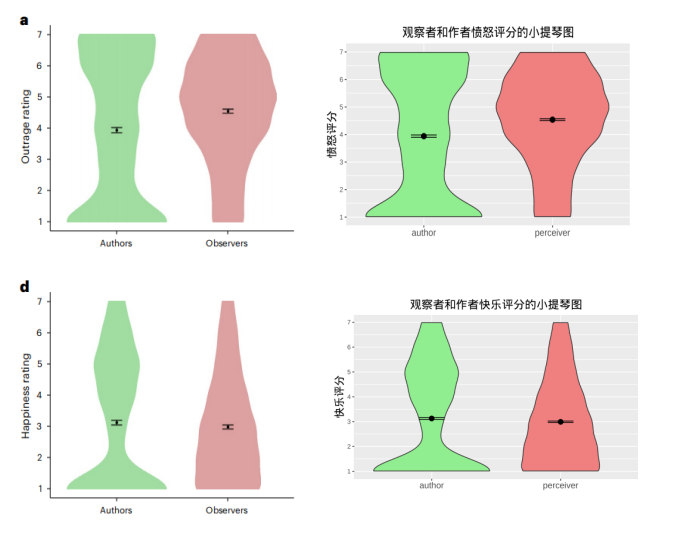
\includegraphics{study1_Violin_Plot.png}
\end{center}
\begin{center}
Figure 1 Reproducibility Results of Descriptive Statistics in Study 1
\end{center}

\hypertarget{inferential-statistics}{%
\subsubsection{Inferential Statistics}\label{inferential-statistics}}

The original study used multilevel modeling to test whether participants tend to overperceive the authors' outrage/happiness. In the multilevel model, the random effects were the tweet authors and participants, the predictor variables were the dummy codes for authors and participants, and the clustering variables were the tweet author IDs and participant IDs. The results showed that the participants' reported levels of outrage were significantly higher than the authors' self-reported levels, indicating that participants had an overperception of outrage, \emph{b} = 0.59, \emph{P} = 0.011, 95\% \emph{CI} {[}0.14, 1.04{]}. However, participants did not overperceive the authors' happiness, \emph{b} = -0.13, \emph{P} = 0.538, 95\% \emph{CI} {[}-0.54, 0.28{]}. The reproduction results were completely consistent with the original study.

\begin{center}
Table 1 Reproducibility test results of study 1 Inferential statistics
\end{center}
\begin{center}
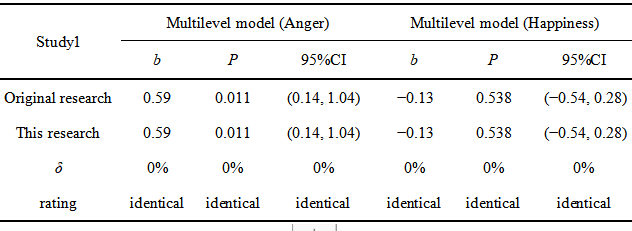
\includegraphics{study1_Reproducibility_Plot.png}
\end{center}

\hypertarget{study-2}{%
\subsection{Study 2}\label{study-2}}

\hypertarget{descriptive-statistics-1}{%
\subsubsection{Descriptive Statistics}\label{descriptive-statistics-1}}

The descriptive statistics of Research 2 are presented in the form of violin plots, as verified for reproducibility using R code. As shown below, figures b and e on the left represent the violin plots from the original literature, while those on the right are generated using self-written R code. From the figures below, it is evident that the shape of the plots generated by the code matches that of the original literature.

\begin{center}
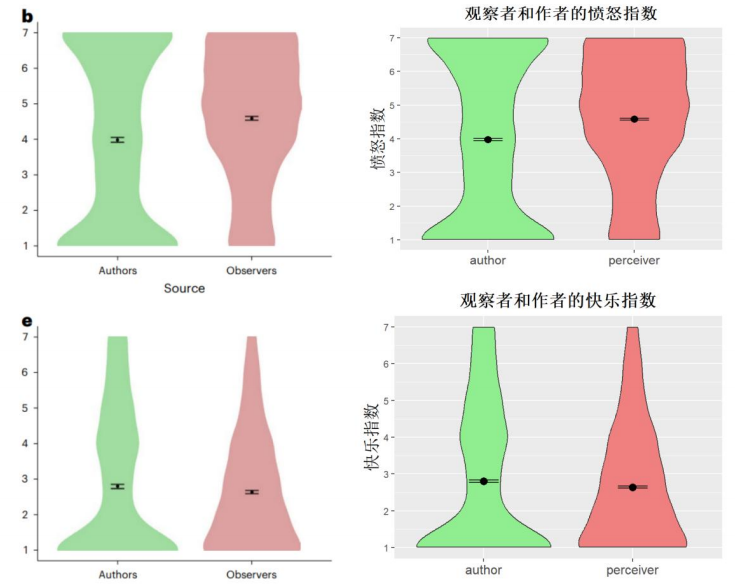
\includegraphics{study2_Violin_Plot.png}
\end{center}
\begin{center}
Figure 2 Reproducibility Results of Descriptive Statistics in Study 2
\end{center}

\hypertarget{inferential-statistics-1}{%
\subsubsection{Inferential Statistics}\label{inferential-statistics-1}}

Research 2 utilized a multilevel modeling approach to investigate whether observers tend to overperceive moral outrage in authors. Random effects included the tweet author and observer, with predictor variables encompassing participant sources (authors and observers) and clustering variables comprising tweet ID and observer ID. Upon comparing the inferential statistical analysis results from the original literature with those reproduced using R code, it was found that the model analysis results closely resembled those of the original literature.

Specifically, observers' perception of outrage was significantly higher than authors, \emph{b} = 0.58, \emph{P} = 0.001, 95\% CI = (0.25, 0.92). Conversely, there was no significant difference in the overperception of happiness between observers and authors, \emph{b} = -0.17, \emph{P} = 0.295, 95\% CI = (-0.49, 0.15). However, there was a minor difference in the confidence interval for happiness scores, where the rounded happiness score computed from the code changed from 0.14 in the original literature to 0.15.

\begin{center}
Table 2 Reproducibility test results of study 2 Inferential statistics
\end{center}
\begin{center}
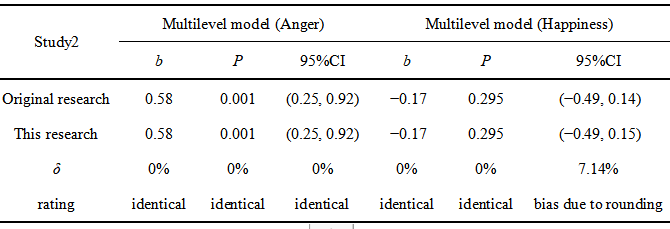
\includegraphics{study2_Reproducibility_Plot.png}
\end{center}

\hypertarget{study-12}{%
\subsection{Study 1\&2}\label{study-12}}

The original study utilized combined data from Research 1 \_ 2 to verify whether participants' political media usage could predict overperception of anger through correlation and regression analyses. It was found that there was a significant positive correlation between the two variables, \emph{r}(222) = 0.19, \emph{P} = 0.004, with a 95\% confidence interval of (0.06, 0.31). Additionally, participants' political media usage significantly predicted overperception of anger, \emph{b} = 0.17, \emph{P} = 0.009. The reproduced results were entirely consistent with the original literature, and scatterplots with regression lines generated using self-written code matched those from the original study (original on the left, self-generated on the right).

\begin{center}
Table 3 Reproducibility test results of study 2 Inferential statistics
\end{center}
\begin{center}
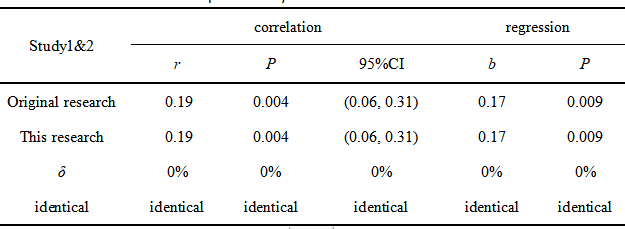
\includegraphics{study1_2_Reproducibility_Plot.png}
\end{center}
\begin{center}
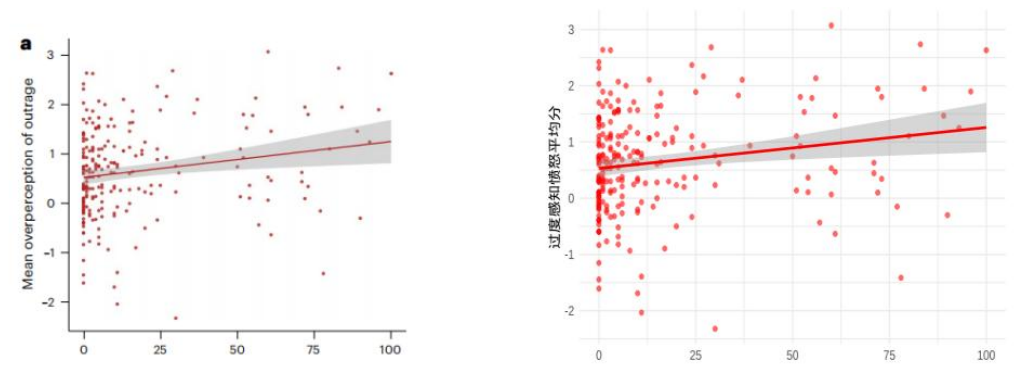
\includegraphics{study1_2_Scatter_Plot.png}
\end{center}
\begin{center}
Figure 3 Reproducibility Results of Descriptive Statistics 
\end{center}

\hypertarget{study-3}{%
\subsection{Study 3}\label{study-3}}

\hypertarget{descriptive-statistics-2}{%
\subsubsection{Descriptive Statistics}\label{descriptive-statistics-2}}

Research 3 utilized the same sample of authors reporting emotions as Research 2, with an increased participant sample size of 350 individuals. Descriptive statistics are presented in violin plots, depicting the distribution of emotions rated by authors (green) and participants (red), similar to Research 1 and 2. Figures on the left display violin plots from the original literature, while those on the right are generated using self-written code. The shape of the plots generated by the code matches that of the original literature, as shown below.

\begin{center}
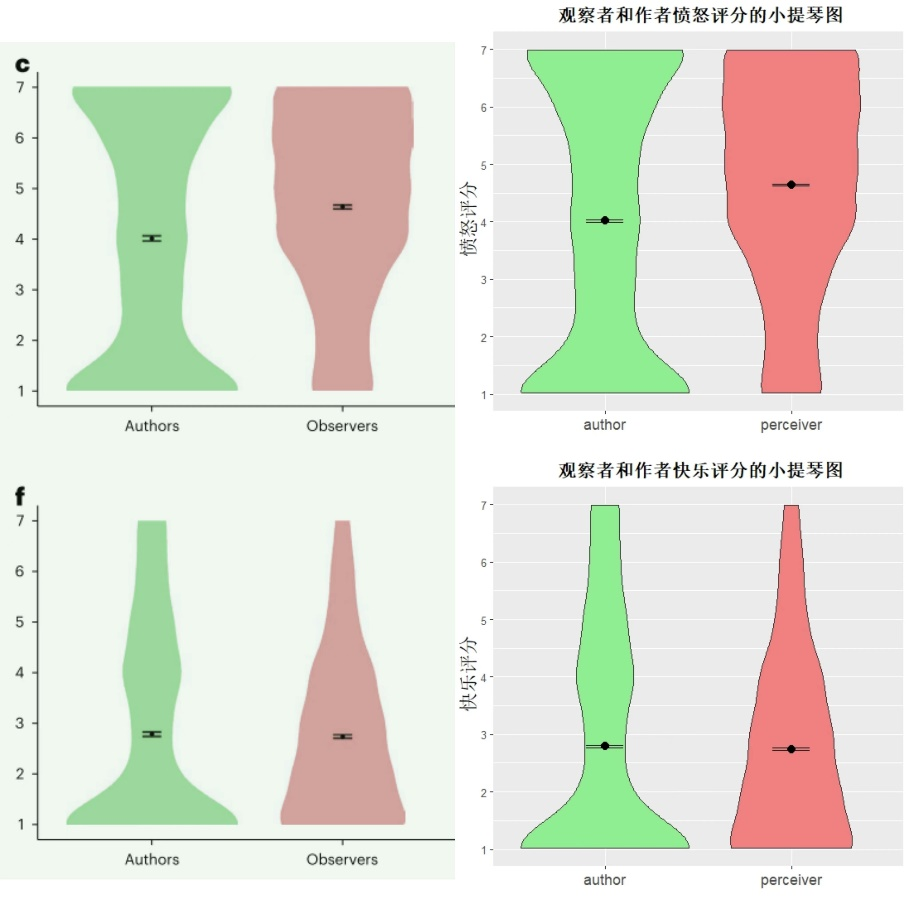
\includegraphics{study3_Violin_Plot.png}
\end{center}
\begin{center}
Figure 4 Reproducibility Results of Descriptive Statistics in Study 3
\end{center}

\hypertarget{inferential-statistics-2}{%
\subsubsection{Inferential Statistics}\label{inferential-statistics-2}}

Research 3 employed a multilevel modeling approach to investigate whether observers tend to overperceive authors' moral outrage. Random effects included tweet author and observer, while predictor variables encompassed participant sources (authors and observers), with tweet ID and observer ID serving as clustering variables. Upon comparing the inferential statistical analysis results from the original literature with those reproduced using R code, it was found that the model analysis results were consistent with the original literature.

Specifically, observers' perception of anger was significantly higher than authors, \emph{b} = 0.62, \emph{P} \textless{} 0.001, 95\% CI = (0.37, 0.88). Conversely, there was no significant difference in the overperception of happiness between observers and authors, \emph{b} = -0.06, \emph{P} = 0.656, 95\% CI = (-0.30, 0.19). However, there were differences in the confidence intervals compared to the original literature, as detailed in the table below.

\begin{center}
Table 4 Reproducibility test results of study 3 Inferential statistics
\end{center}
\begin{center}
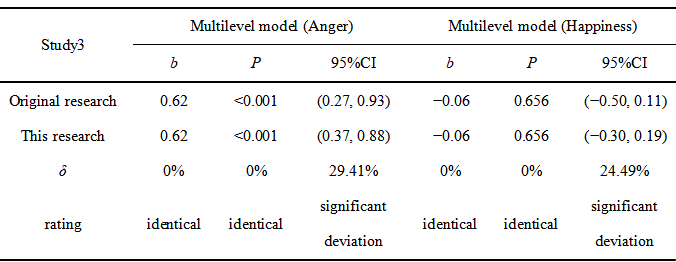
\includegraphics{study3_Reproducibility_Plot.png}
\end{center}

Research 3 also replicated the correlation between overperception of anger and political social media usage, \emph{r}(248) = 0.20, \emph{P} = 0.001, 95\% CI = (0.08, 0.32). Multiple regression analysis adjusted for observers' ideological extremism, partisan identity strength, and tendency to overperceive happiness showed that political social media usage is a significant predictor of overperception of anger. The reproduced results were entirely consistent with the original literature, and scatterplots with regression lines generated using self-written code matched those from the original study (original on the left, self-generated on the right).

\begin{center}
Table 5 Repeatability test results of correlation and regression analysis for study 3
\end{center}
\begin{center}
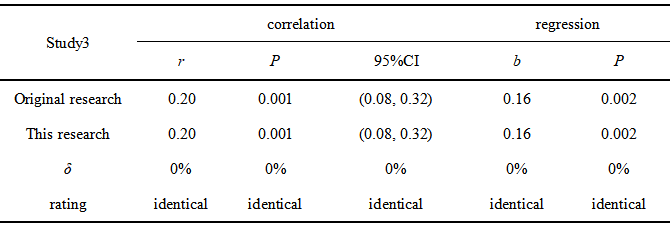
\includegraphics{study3_correlation and regression_Plot.png}
\end{center}
\begin{center}
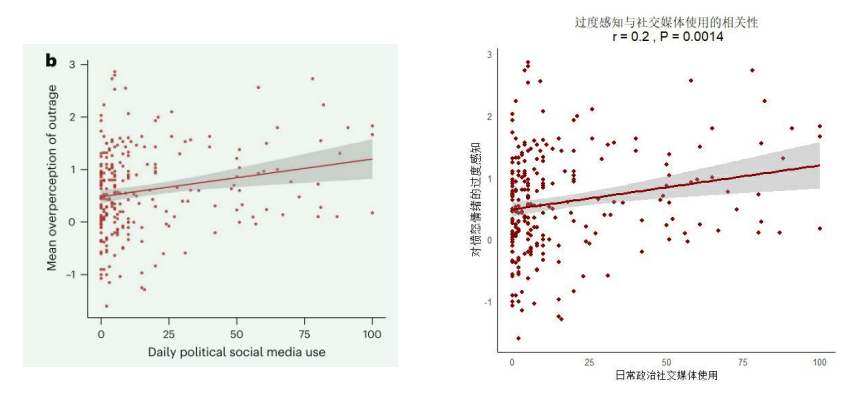
\includegraphics{study3_Scatter_Plot.png}
\end{center}
\begin{center}
Figure 5 Reproducibility Results of scatter plots in Study 3
\end{center}

\hypertarget{study-4-1}{%
\subsection{Study 4}\label{study-4-1}}

\hypertarget{descriptive-statistics-3}{%
\subsubsection{Descriptive Statistics}\label{descriptive-statistics-3}}

Original Study Findings: Recruited 300 Democrats and 300 Republicans. After excluding participants without political party affiliation (\emph{N} = 27) and those who failed comprehension checks (\emph{N} = 52), the final number of participants was 523.

Reproduced Results: The original dataset included a total of 602 participants. After excluding participants without political party affiliation (\emph{N} = 27) and those who failed comprehension checks (\emph{N} = 52), the total number of participants remained 523.

\begin{center}
Table 6 Reproducibility test results of study 4 Inferential statistics
\end{center}
\begin{center}
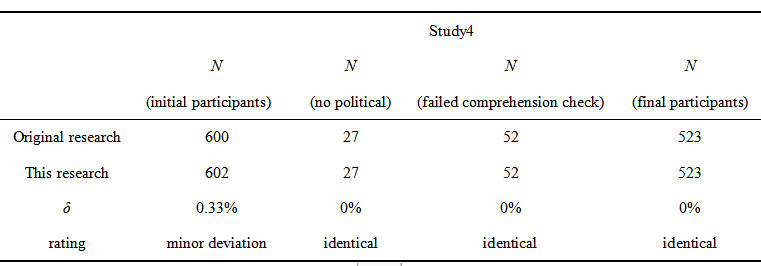
\includegraphics{study4_Reproducibility_Plot.png}
\end{center}

\hypertarget{inferential-statistics-3}{%
\subsubsection{Inferential Statistics}\label{inferential-statistics-3}}

\begin{enumerate}
\def\labelenumi{\arabic{enumi}.}
\tightlist
\item
  Independent Samples t-test
  Original Study Findings: Participants' judgments of collective anger on their social networks under conditions of high overperception of news sources (\emph{M} = 5.82) were significantly higher than judgments under conditions of low overperception of news sources (\emph{M} = 3.53), \emph{t}(479.50) = 21.56, \emph{P} \textless{} 0.001, Cohen's d = 1.90, 95\% CI = (2.09, 2.50).
\end{enumerate}

Reproduced Results: \emph{t} = 21.56, \emph{df} = 479.5, \emph{p} \textless{} 0.001. The mean for the high overperception of tweets group was 5.82, and for the low overperception of tweets group was 3.53. Cohen's d was 1.91, with a 95\% confidence interval for the difference between the means of (2.09, 2.51).

\begin{center}
Table 7 Duplicate results of independent sample t test of study 4
\end{center}
\begin{center}
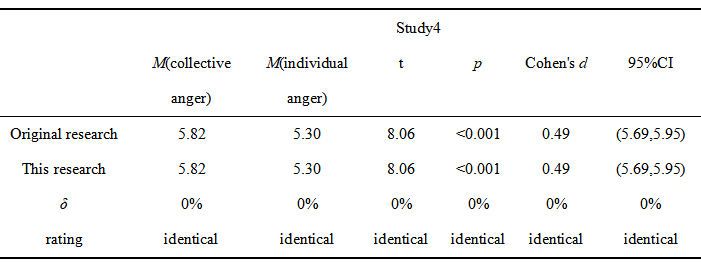
\includegraphics{study4_independent_test_Plot.png}
\end{center}

\hypertarget{single-sample-t-test}{%
\paragraph{Single-Sample t-test}\label{single-sample-t-test}}

\begin{enumerate}
\def\labelenumi{\arabic{enumi}.}
\setcounter{enumi}{1}
\tightlist
\item
  High Overperception of Tweets Group
  Original Study Findings: Under conditions of high overperception, participants' perception of
  collective anger (\emph{M} = 5.82) was significantly greater than the perceived anger mean (\emph{M} =5.30)
  when viewing each news source individually, \emph{t}(264) = 8.06, \emph{P} \textless{} 0.001, \emph{d} = 0.49, 95\% CI = (5.69, 5.95).
  Reproduced Results: \emph{t} = 8.01, \emph{df} = 264, \emph{p} \textless{} 0.001, 95\% CI = (5.69, 5.95), Cohen's d = 0.49. The mean perception of collective anger was 5.82, while the mean perception of anger when viewing each news source individually was 5.30.

  \begin{center}
  Table 8 Single-Sample t-test (High Overperception of Tweets)
  \end{center}
  \begin{center}
  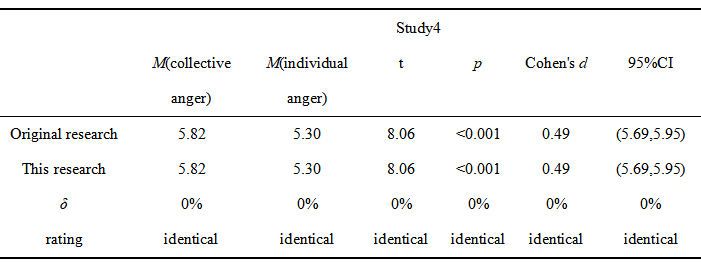
\includegraphics{study4_Single-Sample_high.png}
  \end{center}
\item
  Low Overperception of Tweets Group
  Original Study Findings: Under conditions of low overperception, participants' perception of collective anger did not differ significantly from the perceived anger mean when viewing each news source individually, \emph{t}(252) = 1.38, \emph{P} = 0.169, \emph{d} = 0.09, 95\% CI = (3.36, 3.69).
\end{enumerate}

Reproduced Results: \emph{t} = 1.38, \emph{df} = 252, \emph{p} = 0.169, 95\% CI = (3.36, 3.69), Cohen's d = 0.09. The mean perception of collective anger was 3.53, while the mean perception of anger when viewing each news source individually was 3.41.

\begin{center}
Table 9 Single-Sample t-test (low Overperception of Tweets)
\end{center}
\begin{center}
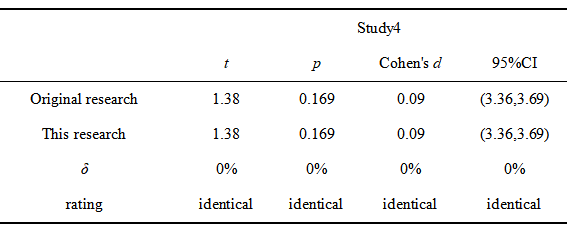
\includegraphics{study4_Single-Sample_low.png}
\end{center}

Finally, visualize observers' perceptions of collective anger under two different conditions (high overperception and low overperception). Use a dashed line to represent the mean perception of individual anger by observers, points for observers' perceptions of collective anger, and bars for the mean perception of collective anger. Ensure that the shape of the generated plot matches that of the original literature (left: original plot,right: generated plot).

\begin{center}
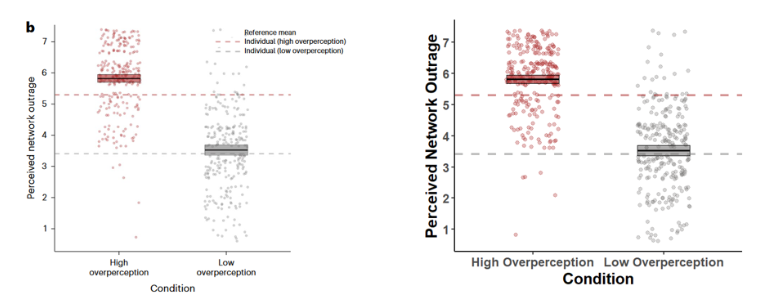
\includegraphics{study4_Visualized_Plot.png}
\end{center}
\begin{center}
Figure 6 Visualized repeatable test results in Study 4
\end{center}

\hypertarget{study-5-1}{%
\subsection{Study 5}\label{study-5-1}}

\hypertarget{descriptive-statistics-4}{%
\subsubsection{Descriptive Statistics}\label{descriptive-statistics-4}}

Researchers recruited 600 Democrats and 600 Republicans to participate jointly in a preregistered study on making social judgments {[}\url{https://osf.io/mjftk}{]}. On the OSF platform, researchers reported how they determined sample size, data exclusion criteria, and all measurement methods. In this study, participants without political party affiliation (N = 100) and those who failed comprehension checks (\emph{N} = 87) were excluded, resulting in a final sample size of \emph{N} = 1013. Replication results were consistent with the original study findings.

\begin{center}
Table 10 Descriptive Statistics of Participant Replication Results
\end{center}
\begin{center}
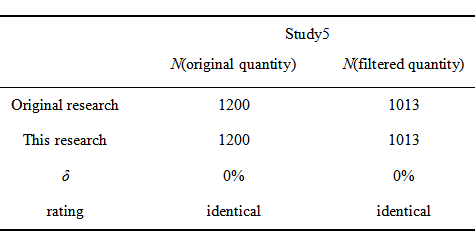
\includegraphics{descriiptive_5.png}
\end{center}

In Study 5, the researchers computed frequencies for gender, party affiliation, and familiarity, and created histograms for age distribution and political ideology. The original study did not provide mean and standard deviation for age, only histograms of age distribution. In the replication, the mean age was calculated as \emph{M} = 36.96, with a standard deviation of \emph{SD} = 13.95.

According to the author's provided code, the frequency for Democrats was 533, accounting for 52.67\% of the total participants; the frequency for Republicans was 479, accounting for 47.33\% of the total participants. Ideological histograms were generated based on the provided code.

\begin{center}
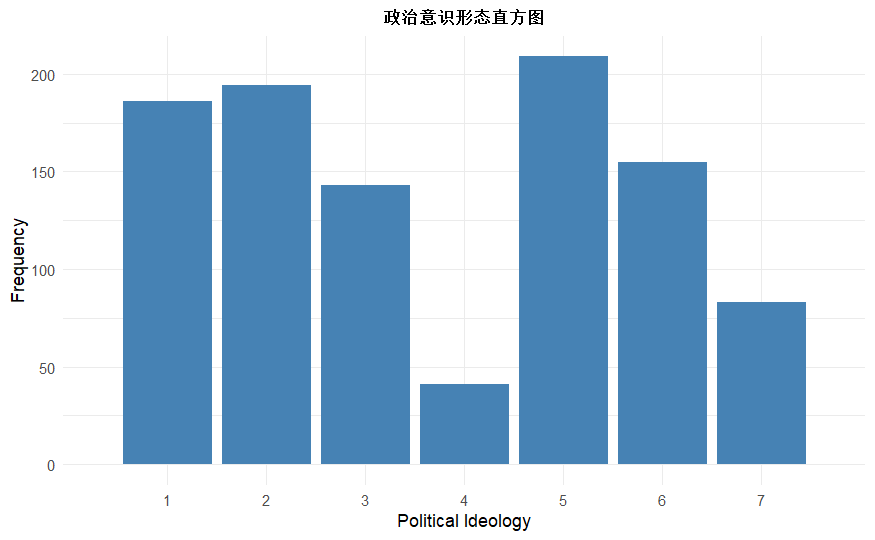
\includegraphics{political_5.png}
\end{center}
\begin{center}
Figure 7 Political Ideology Histogram in Study 5
\end{center}

\hypertarget{inferential-statistics-4}{%
\subsubsection{Inferential Statistics}\label{inferential-statistics-4}}

\begin{enumerate}
\def\labelenumi{\arabic{enumi}.}
\tightlist
\item
  Perception of Anger across Different News Input Groups
  Researchers analyzed the distribution, homogeneity of variance, significance, and effect size of data under conditions of high and low perception of anger. The sign of the t-value indicates the direction of the mean difference between the two groups. The original results showed: \emph{t}(964.58) = −6.89, \emph{p} \textless{} 0.001, \emph{d} = 0.43, 95\% CI = (0.47, 0.85); our replication results showed: \emph{t}(964.58) = 6.89, \emph{p} \textless{} 0.001, \emph{d} = 0.43, 95\% CI = (0.47, 0.85). Except for the sign of the t-value, our results are consistent with the original study. A positive t-value indicates that the appropriateness scores of the high perception group are higher than those of the low perception group, suggesting that the high perception group perceives anger as more suitable for society.

  \begin{center}
  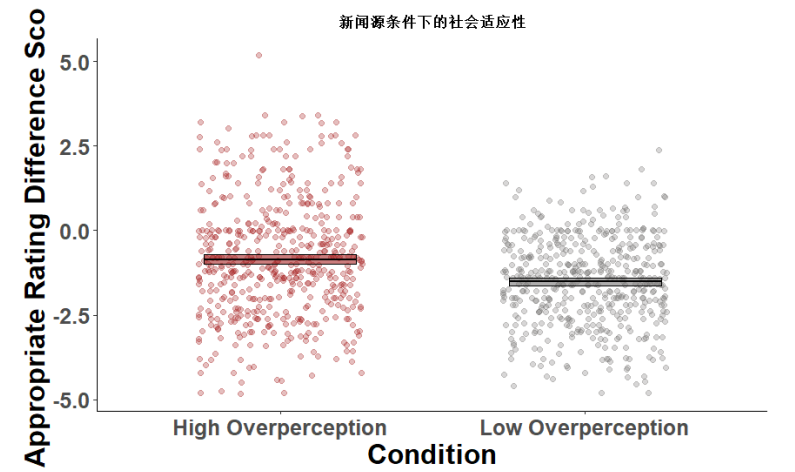
\includegraphics{fitness_5.png}
  \end{center}
  \begin{center}
  Figure 8 Social Adaptability under the Conditions of News Sources in Study 5
  \end{center}
  \begin{center}
  Table 11 Description of the Number of Participants with Repetition Results Statistics in Study 5
  \end{center}
  \begin{center}
  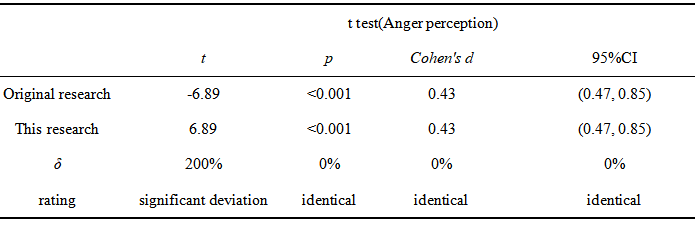
\includegraphics{table12_repeat.png}
  \end{center}
\item
  Does perceived anger amplify group polarization?
  The original results found that the analysis of variance showed a significant interaction between conditions and online networks, \emph{F}(1, 1010) = 369.58, \emph{p} \textless{} 0.001, n\_\{2\}\^{}\{p\} = 0.27. Participants who viewed news from highly anger-inducing sources expressed greater liking for their political in-group compared to those who viewed news from sources inducing lower levels of anger (\emph{p} \textless{} 0.001). Participants who viewed news from highly anger-inducing sources also reported higher dislike for political out-groups on their social networks, whereas those who viewed news from sources inducing lower anger reported lower dislike for political out-groups, with significant differences between the two groups (\emph{p} \textless{} 0.001). Post hoc tests indicated that the effect of news source condition on increasing dislike for political out-groups was nearly twice as strong as its effect on increasing liking for political in-groups. These findings suggest that when individuals perceive excessive anger in news sources, they tend to perceive a significant emotional polarization in their social networks. Our test results align with the original findings, where the analysis of variance showed \emph{F}(1, 1010) = 369.58, \emph{p} \textless{} 0.001, n\_\{2\}\^{}\{p\} = 0.27. The source code did not successfully produce results or statistical figures, and did not include the post hoc test section, which was also absent from the original manuscript. After modifying the code, the following figure was obtained.

  \begin{center}
  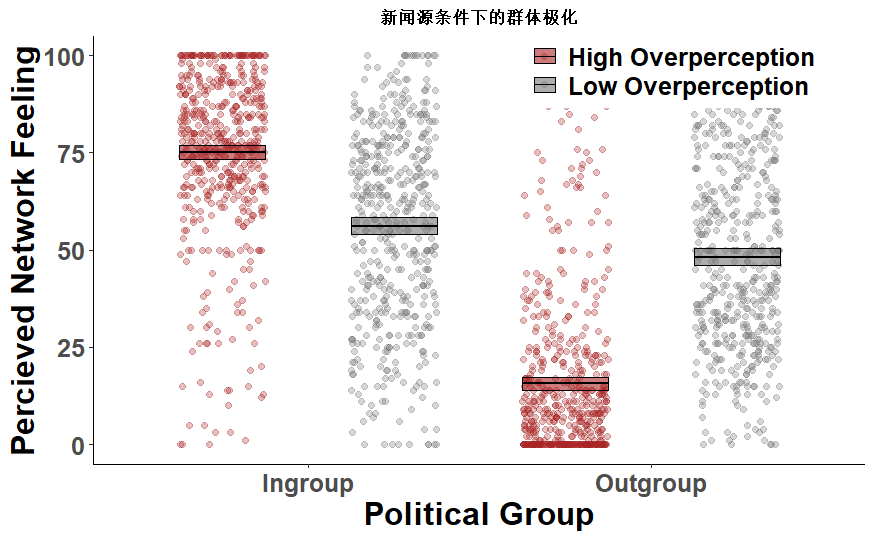
\includegraphics{quntijihua_5.png}
  \end{center}
  \begin{center}
  Figure 9 Group Polarization under News Source Conditions in Study 5
  \end{center}
  \begin{center}
  Table 12 Results of F-test (Group Polarization) in Study 5
  \end{center}
  \begin{center}
  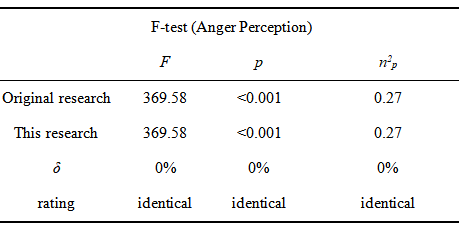
\includegraphics{Results_F.png}
  \end{center}
\item
  The impact of anger perception on group polarization
  In the original study, researchers found that compared to participants who viewed news from sources inducing lower levels of anger, those who viewed news from sources inducing higher levels of anger perceived their networks to be more ideologically extreme, \emph{t}(1003.60) = -11.39, \emph{p} \textless{} 0.001, \emph{d} = 0.72, 95\% CI = (0.46, 0.64). Replication results closely aligned with the original findings, except for a discrepancy in the sign of the t-value, which was \emph{t}(1003.60) = 11.39, \emph{p} \textless{} 0.001, \emph{d} = 0.72, 95\% CI = (0.46, 0.64). Integrating findings from Study 5 suggests that excessive perception of anger in news sources directly amplifies perceptions of norms for expressing anger, emotional polarization, and ideological extremism in social networks.

  \begin{center}
  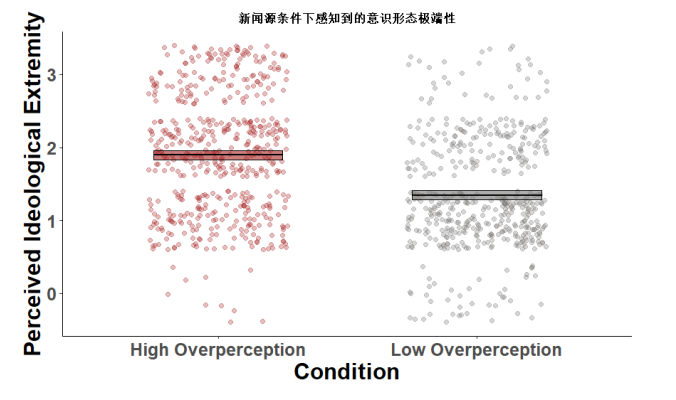
\includegraphics{study5_3.png}
  \end{center}
  \begin{center}
  Figure 10 Perceived Ideological Extremity under News Source Conditions in Study 5
  \end{center}
  \begin{center}
  Table 13 Test Results (Ideological Extremity) in Study 5
  \end{center}
  \begin{center}
  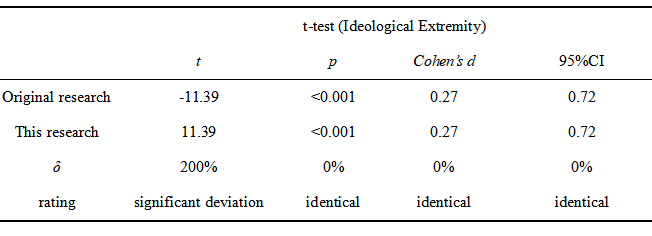
\includegraphics{test_result.png}
  \end{center}
\end{enumerate}

\hypertarget{summary-and-discussion}{%
\section{Summary and Discussion}\label{summary-and-discussion}}

\hypertarget{reproducibility-assessment-in-the-original-study}{%
\subsection{Reproducibility Assessment in the Original Study}\label{reproducibility-assessment-in-the-original-study}}

\begin{center}
Table 14 Analysis of Reasons for Non-reproducibility
\end{center}
\begin{center}
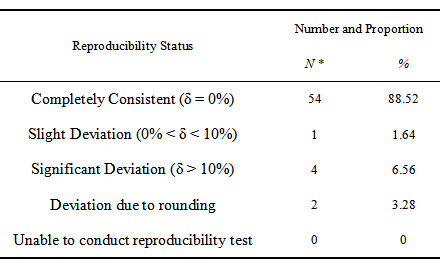
\includegraphics{reproducibility.png}
\end{center}

In this reproducibility study, we identified several instances where results deviated or could not be replicated. These issues primarily centered around the following areas. Firstly, some results could not be replicated due to incomplete data or insufficient information provided in the original paper. For example, age data of participants were not disclosed in the original paper, making comparisons impossible. Secondly, discrepancies arose from inconsistencies between the original data and code files. This included operations in the code that lacked corresponding data entries, complicating the replication process. Additionally, ambiguities were found in the procedural reporting, such as unclear or incorrect reporting of variables used in regression models and criteria for subgroup inclusion. Descriptive statistics also exhibited deviations; for instance, the reported original participant count of 600 individuals in the paper differed from the actual count of 602 individuals in the dataset, impacting the analysis process. In the statistical inference part, rounding discrepancies were noted; for example, the confidence interval for happiness index in Study 2 shifted from 0.14 as reported in the paper to 0.15 due to rounding, affecting the interpretation of results. Some confidence intervals or effect sizes also differed slightly from the original paper; for instance, Study 3 showed variations in confidence intervals between observers and authors in the perception of excessive happiness.
Furthermore, discrepancies in the sign of statistical test values were observed; for example, in Study 4, although the numerical value of the t-statistic was consistent, the opposite sign indicated a different direction in the mean differences between groups.
While most results aligned with the original paper during replication, these minor deviations in critical findings underscore the need for rigorous validation. These findings emphasize the importance of transparent data and code sharing practices, as well as detailed reporting in academic research to enhance reproducibility and credibility.

\hypertarget{analysis-of-reproducibility-test-results}{%
\subsection{Analysis of Reproducibility Test Results}\label{analysis-of-reproducibility-test-results}}

For Study 3, the inconsistent confidence interval results can be attributed to differences in sample sizes and data collection procedures compared to Studies 1 and 2. Additionally, the absence of a random seed setting in Study 3's data collection process may have contributed to these discrepancies.
In the descriptive statistics section of Study 4, regarding participant numbers, the original paper reported 600 participants, while the dataset actually contained 602 participants, and all analyses were conducted based on the latter number. This discrepancy is suspected to be an authorial error, impacting reproducibility.
In Study 5, the original code encountered issues and could not run smoothly. We made modifications to the ``mutate'' function within ``descriptives,'' specifically changing the levels from ``Over perception'' and ``Accurate Perception'' to ``High Overperception'' and ``Low Overperception.'' This modification was necessary because the data did not contain columns labeled ``Over perception'' and ``Accurate Perception.''
These issues may also stem from problems with code modifications, authorial errors, software package or version issues, or delayed updates by the original authors.

\hypertarget{further-reflections}{%
\subsection{Further Reflections}\label{further-reflections}}

In terms of course learning, this reproducibility study deepened our understanding of R programming and statistical methods, particularly in handling complex datasets and conducting multilevel model analyses practically. Moreover, in scientific research, we gained insights into research methodologies and recognized the importance of transparent data and detailed reporting in ensuring the reliability and reproducibility of research results. Regarding teamwork, this project enhanced our collaborative and communication skills, ensuring smooth project progress through clear division of labor and mutual support.
Finally, concerning coursework, the integration of practical tasks with theoretical learning equipped us not only with technical skills but also fostered critical thinking, which is crucial for future research endeavors. We suggest that courses include more practical components to better assist students in understanding and applying the knowledge they acquire.

\newpage

\hypertarget{references}{%
\section{References}\label{references}}

Brady, W. J., McLoughlin, K. L., Torres, M. P., Luo, K. F., Gendron, M., \& Crockett, M. J. (2023). Overperception of moral outrage in online social networks inflates beliefs about intergroup hostility. \emph{Nature Human Behaviour}. \url{https://doi.org/10.1038/s41562-023-01582-0}

\hypertarget{refs}{}
\begin{CSLReferences}{0}{0}
\end{CSLReferences}


\end{document}
